\documentclass{standalone}
\usepackage{tikz}
\usepackage{tikzscale}
\usetikzlibrary{arrows}
\usetikzlibrary{arrows.meta}
\usetikzlibrary{patterns}
\usetikzlibrary{shapes}
\usetikzlibrary{calc}
\usetikzlibrary{matrix}
\usetikzlibrary{positioning}
\usepackage{calc}
\usetikzlibrary{calc,trees,positioning,arrows,fit,shapes}

\usepackage{tkz-euclide}
\usetikzlibrary{
	angles,
	quotes,
}
\usepackage{pgfplots}
\begin{document}

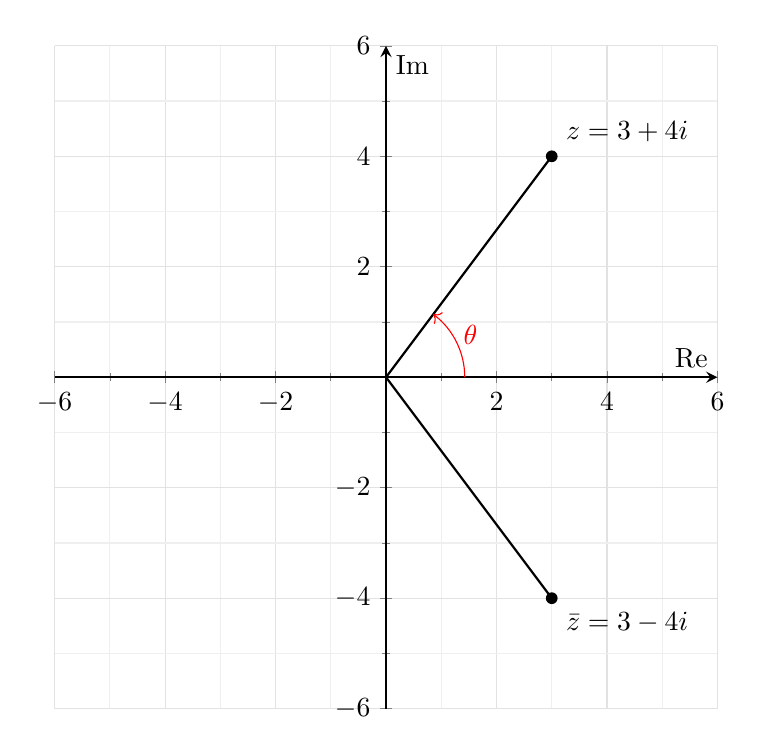
\begin{tikzpicture}
	\begin{axis}[
		xmin = -6, xmax = 6,
		ymin = -6, ymax = 6,    
		grid = both,
		minor tick num = 1,        
		axis lines=center,
		axis line style = thick,          
		major grid style = {lightgray!45},
		minor grid style = {lightgray!25},  
		xlabel = {Re},
		ylabel = {Im},
		disabledatascaling,
		axis equal,
		width=10cm,
		height=10cm	        
		]
		\node[label={45:$z=3+4i$},circle,fill,inner sep=1.5pt] (A) at (axis cs:3,4) {};  
		\node[label={-45:$\bar{z}=3-4i$},circle,fill,inner sep=1.5pt] () at (axis cs:3,-4) {};        
		\addplot[domain = 0:3,	thick, 	black, ] {4*x/3};
		\addplot[domain = 0:3,	thick, 	black, ] {-4*x/3};
		
		\coordinate (xaxis) at (\pgfkeysvalueof{/pgfplots/xmax},0);
		\coordinate (origin) at (0,0);
		%\addplot [->,blue] coordinates {(0, 0) (2, 3)} coordinate [at end] (A) ;
		\path (xaxis) -- (origin) -- (A)
		pic [
		draw,
		->,
		red,
		angle radius=10mm,
		angle eccentricity=1.2,
		"$\theta$",
		] {angle = xaxis--origin--A}
		;
	\end{axis}
\end{tikzpicture}


\end{document}
